\documentclass[12pt]{article}
\pagenumbering{arabic}
%\textwidth 16cm
%\textheight 22.7cm
%\topmargin -0.7cm
%\oddsidemargin 0.45cm
%\evensidemargin 0.6cm
%\leftmargin -1.0cm
%\rightmargin 0.0cm
\pagestyle{plain}
\usepackage{graphicx}

\begin{document}
  \begin{titlepage}
  \begin{center}
\vbox{}

    \vspace{30mm}

    {\Huge  XGEN}\\[6mm]

Simple triangular mesh generator based on the Advanced Front method,\\
implemented in X-Windows using the Motif library.

    \vspace{20mm}

\begin{center}
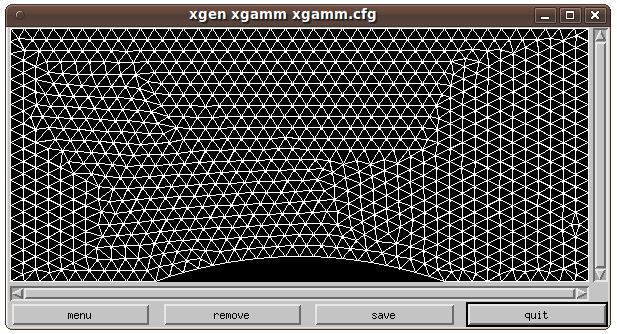
\includegraphics[width=0.8\textwidth]{xgamm.png}
\end{center}
    \vspace{20mm}

    Version 6.0\\
    \copyright 2010 $hp$-FEM group, University of Nevada, Reno\\
    Email: hpfem-group@googlegroups.com. Home page: http://hpfem.org.

  \end{center}
  \end{titlepage}

  \section{Introduction}

  The interactive grid generator XGEN makes it possible,
  after writing a short C++ application, to generate unstructured
  triangular grids on arbitrary polygonal domains. 
  The user enters a positively oriented boundary,
  XGEN calculates the area of the domain, and throws inside an
  appropriate number of random points. Then an electrostatics simulation 
  evolves the points until they reach an equilibrium. 
  The user can add and remove points using the left and right mouse click,
  respectively. At any time the user can click a Grid button and 
  triangulate the point set.

  \section{Getting started} \label{getting}
  
  Prerequisites include the Motif library. In Ubuntu install it using:

\begin{verbatim}
  sudo apt-get install libmotif-dev libmotif3 lesstif2
\end{verbatim}
  Then install XGEN by typing ``make''. The present Makefile works for
  Ubuntu Linux, but it should work on other Linux and Unix platforms with 
  minor modifications.
  
  When creating a new project, the user has to write 
  a few lines of a simple C++ code that define a new descendant of
  a basic class Xgen. For example, let us create a class ``xsquare''
  that will just triangulate a square domain. We add the following 
  code to other project classes defined in the file {src/xmain.cpp}:

  \footnotesize
  \begin{verbatim}
class xsquare: public Xgen {
  public:
  xsquare(char *cfg_filename) : Xgen() {XgInit(cfg_filename);}
  virtual void XgReadData(FILE *f);
};

void xsquare::XgReadData(FILE *f) {
  int N; 
  if(!Get(f, &N)) XgError("Couldn't read N.");
  XgAddEdge(3, 0, 0, N);
  XgAddEdge(2, 1, 0, N);
  XgAddEdge(4, 1, 1, N);
  XgAddEdge(1, 0, 1, N);
}
  \end{verbatim}
  That's it. This tells XGEN to create a unit square domain with four edges. The first 
  edge with boundary marker '3' starts at [0, 0] and it is subdivided 
  equidistantly into 'N' intervals. An edge ends where the next one  
  starts and the end of the last edge is the starting point of the first one.
  Later we will learn how to create loops (holes) in the domain.\\
  
  \noindent
  The function Get(FILE *, ...) is overloaded for all useful types. 
  The symbol \# introduces a comment.\\

  \noindent
  Every project needs to have a configuration file with 
  geometry parameters. For example, the class xsquare only 
  uses one integer number 'N', and thus the corresponding 
  configuration file xsquare.cfg looks as follows:
  \begin{verbatim}  
# a cfg file to the class 'xsquare'
# subabscissas at one side of the square:
15
  \end{verbatim}
  This file can be found in the actual directory. \\

  \noindent
  The square domain is then triangulated by running xgen with the 
  project xsquare and the configuration file name as command-line 
  parameters:

  \begin{verbatim}  
  xgen xsquare cfg/xsquare.cfg
  \end{verbatim}
  If you like, you can use additional Motif options such as:

  \begin{verbatim}  
  xgen xsquare cfg/xsquare.cfg -bg lightgray -fg blue 
  \end{verbatim}
  For a list of all possible options see the Motif1.2 Reference Guide.\\

  \noindent
  After running xgen you should see a graphical window with 
  points moving inside. You can add and remove points using 
  the left and right mouse buttons, respectively. The roles of 
  the buttons are self-explanatory. 

  \section{Mesh output format} \label{out_form}

  XGEN writes meshes in the Hermes2D native format (http://hpfem.org/hermes).
  To override it for your project, redefine the virtual method XgUserOutput().\\

  \noindent
  Example: with the configuration file 

  \begin{verbatim}
# This is a cfg file to the class 'xsquare'
# Number of subabscissas at one side of the square:
2  
  \end{verbatim}
  each side of the square consists of two domain boundary edges. Calling XGEN, the generator
  only inserts one point into the domain. Resulting grid file looks like
  \begin{verbatim}
# XGEN mesh in Hermes2D format
# Project: xsquare
# Edges are positively oriented

# Vertices:
vertices = 
{
  { 0, 0 },
  { 0.5, 0 },
  { 1, 0 },
  { 1, 0.5 },
  { 1, 1 },
  { 0.5, 1 },
  { 0, 1 },
  { 0, 0.5 },
  { 0.499998, 0.499998 }
}

# Elements:
# (three vertex indices and a '0' (dummy material marker))
elements =
{
  { 7, 0, 8, 0 },
  { 8, 0, 1, 0 },
  { 8, 1, 3, 0 },
  { 3, 1, 2, 0 },
  { 8, 3, 5, 0 },
  { 5, 3, 4, 0 },
  { 8, 5, 7, 0 },
  { 7, 5, 6, 0 }
}

# Boundary data:
# (bdy_vrt_1 bdy_vrt_2 edge_index)
boundaries =
{
  { 0, 1, 3 },
  { 1, 2, 3 },
  { 2, 3, 2 },
  { 3, 4, 2 },
  { 4, 5, 4 },
  { 5, 6, 4 },
  { 6, 7, 1 },
  { 7, 0, 1 }
}
  \end{verbatim}

  \section{Saving and loading points}

  Sometimes you may need to conserve grid point coordinates for
  further use. In ``menu'', you can use the button ``save points''.
  To load points, use buttons ``init'' and ``load''.
  \indent
  The output file only contains points coordinates, i.e. two
  doubles per line. Reading of points finishes when end of file
  or an error while reading. Points which are checked to be
  out of the domain are ignored. This way, if you prepare a 
  special point file with ordered points, it may take less
  time to the generator to get near the minimal potential.  

  \section{XGEN configuration file}
   
  After calling XGEN, the generator tries to open file
  .XgenConfig in the current directory. If it is succesful,
  it tries to read as much information as possible in the
  following format:

  \begin{verbatim} 
# Point file path:
points/
# Grid file path:
meshes/
# SubLoopsNumber:
100
# Initial size limit:
600
# Boundary redraw interval:
200
# TimestepConst:
0.707
# ZoomConst:
0.95
  \end{verbatim}
  Variables which are not read remain set to implicitly defined
  values. Point and grid file paths say, where the point and grid 
  files are to be stored, respectively. SubLoopsNumber is the number of
  points to be moved before returning control to the Window Manager.
  The next value is the size of the window when placed onto the screen.
  You may notice that its shape is determined according to the shape
  of the triangulated domain by the generator itself. BoundaryRedrawInterval
  is the number of points to be moved before the boundary will be
  redrawn. TimestepConst is a number between 0 and 1 expressing the change of
  the time-step after pressing ``timestep inc'' and ``timestep dec'' in ``menu''.
  The same meaning has the last value of the file in the sense of
  zooming the domain.

  \section{Visualization of meshes}

  In the subdirectory meshes/ there is a file ``tognu.cpp'' which,
  after having installed it
  \begin{verbatim}
  gcc -o tognu tognu.cpp -lm
  \end{verbatim}
  enables to prepare Gnuplot--format files of XGEN grids. It must be called with
  two command-line arguments: the grid file name and the output Gnuplot--format file
  name, i.e. for example
  \begin{verbatim}
  tognu xsquare.grid xsquare.gnu
  \end{verbatim}
  Then Gnuplot can be used for the visualization of XGEN grids.

  \section{Creating user applications} \label{vl_apl}

  The class Xgen is defined as an empty class. It knows all algorithms
  necessary for moving points and creating grids but it knows nothing
  about the domain. The domain is passed into the generator in virtue of
  its descendants. You have to redefine the virtual method

  \begin{verbatim}
    virtual void XgReadData(FILE *f) = 0;
  \end{verbatim}

  \noindent
  and, in addition, you can also redefine the methods
  \begin{verbatim}
    virtual double XgCriterion(Point a, Point b, Point c);
    virtual void XgUserOutput(FILE *f);
  \end{verbatim}
  The example ``xsquare'' from the section \ref{getting} explains, how the redefinition is carried out.

  \section{Redefining the method XgReadData()}

  First, we introduce definition of a useful structure ``Point'' which is
  used by the generator:
  \begin{verbatim}
struct Point {
  double x, y;

  Point() {}
  Point(double ix, double iy): x(ix), y(iy) {}
  double abs() {return sqrt(x*x + y*y);}

  Point &operator += (Point B) {x += B.x; y += B.y; return *this;}
  Point &operator -= (Point B) {x -= B.x; y -= B.y; return *this;}
  Point &operator *= (double k) {x *= k; y *= k; return *this;}
  Point &operator /= (double k) {x /= k; y /= k; return *this;}
  Point &operator *= (int k) {x *= k; y *= k; return *this;}
  Point &operator /= (int k) {x /= k; y /= k; return *this;}
  Point operator + (Point B) {return Point(x + B.x, y + B.y);}
  Point operator - (Point B) {return Point(x - B.x, y - B.y);}
  Point operator * (double k) {return Point(k*x, k*y);}
  Point operator / (double k) {return Point(x/k, y/k);}
  Point operator * (int k) {return Point(k*x, k*y);}
  Point operator / (int k) {return Point(x/k, y/k);}
  double operator * (Point B) {return x*B.x + y*B.y;}
};
  \end{verbatim}  
  The method XgReadData() is given pointer to the descendant's configuration
  file (e.g. to ``xsquare.cfg'') which has been open for binary reading. The pointer
  is NULL if the opening failed. User-defined XgReadData() must read from this
  file all parameters characterizing the domain in order to fill the descendant's 
  data. Shape of the domain is passed into the descendant by means of the following
  overloaded method:
  \begin{verbatim}
    void XgAddEdge(int index, double x, double y);
    void XgAddEdge(int index, Point P);
    void XgAddEdge(int index, double x, double y, int lines);
    void XgAddEdge(int index, Point P, int lines);
  \end{verbatim}
  This method adds one edge to the Xgen data structure representing the
  boundary of the triangulated domain. The boundary must be positively
  oriented. The value ``index'' means the user-defined kind of the
  corresponding boundary part (see the output format in \ref{out_form}).
  The coordinates ``x, y'' or the point ``P'' is the starting point of the edge.
  The number ``lines'' means the number of boundary edges the edge will be
  equidistantly divided into. The end point of the edge is determined either
  by adding another edge (then it is its starting point) or by calling 
  \begin{verbatim}
    void XgNewComponent();
  \end{verbatim}
  which closes the loop. Last given loop is closed automatically. You make take profit
  of the function
  \begin{verbatim}
    int Get(FILE *f, Point *what);
  \end{verbatim}
  which reads a Point (i.e. two double coordinates).

  \section{Additional examples}

  The executable file ``xgen'' (see its source in src/xmain.cpp) contains
  some more example descendants -- there are ``xcirc'', ``xhole'', ``xgamm'', 
  ``xstep'' and ``xlist''. Run them analogously as the ``xsquare'' in \ref{getting}:
  \begin{verbatim}
    xmain xsquare xsquare.cfg &
    xmain xhole xhole.cfg &
    xmain xcirc xcirc.cfg &
    xmain xhump xhump.cfg &
    xmain xstep xstep.cfg &
    xmain xlist xlist.cfg &
  \end{verbatim}

  \section{Redefinition of the method XgCriterion()}

  This method is important for the triangulation of the domain. The algorithm solves
  the following task: let $ab$ be an oriented edge, points $c_1, c_2, \ldots, c_k$ lie on the left
  hand side of $ab$ (this can be written precisely). We want to choose a point $c_i$ from them
  so that the triangle
  $abc_i$ is ``the nicest one possible'' and none from the rest of points $c_j$, 
  $ i \not= j$, $j = 1, 2, \ldots, k$ lies inside of $abc_i$. Having two different
  triangles, by means of ``XgCriterion()'' we define, which one of them is nicer -- its XgCriterion
  is smaller. Each defined XgCriterion() must satisfy the following implication:
  XgCriterion(a, b, c) $<$ 
  XgCriterion(a, b, d) then the point $d$ lies outside of the triangle $abc$ for all $c, d$ lying
  on the left of $ab$.
  The implicit definition of XgCriterion(a, b, c) is

  \begin{verbatim}
double Xgen::XgCriterion(Point a, Point b, Point c) {
  return ((c-a)*(c-b))/((c-a).abs()*(c-b).abs());
}
  \end{verbatim}
\hbox{} \hfill Pavel Solin, May 1995 (updated November 2010)


\end{document}






